\begin{figure}
\centering

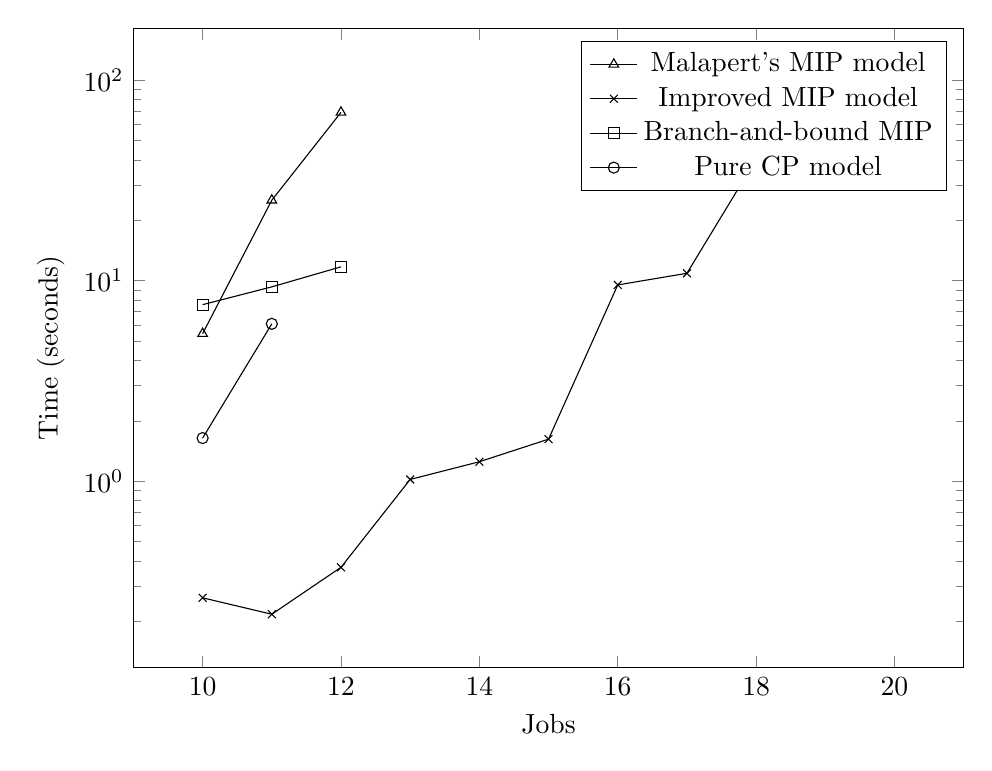
\begin{tikzpicture}
  \begin{semilogyaxis}[xlabel=Jobs, ylabel=Time (seconds), width=\textwidth,
  height=0.8\textwidth]
  \addplot[color=black, mark=triangle ] coordinates { % MIP model times
  (10, 5.441)
  (11, 25.18)
  (12, 69.05)
  };   \addlegendentry{Malapert's MIP model}

  \addplot[color=black, mark=x ] coordinates { % MIP model times
  (10, 0.262)
  (11, 0.217)
  (12, 0.372)
  (13, 1.02)
  (14, 1.25)
  (15, 1.62)
  (16, 9.52)
  (17, 10.88)
  (18, 40.3)
  (19, 42.5)
  (20, 98.415)
  };   \addlegendentry{Improved MIP model}

  \addplot[color=black, mark=square] coordinates {
(10, 7.59)
(11, 9.31)
(12, 11.72)
  };
  \addlegendentry{Branch-and-bound MIP}
  \addplot[color=black, mark=o] coordinates {
(10, 1.64)
(11, 6.09)
};
  \addlegendentry{Pure CP model}
  \end{semilogyaxis}
\end{tikzpicture}

\caption{Comparison of CPU time used by different models to find an optimal
schedule and prove its optimality.}
\label{fig:comp_times}
\end{figure}

